
\section{Plots Normalized by Area}

\begin{figure}[h]
  \centering
  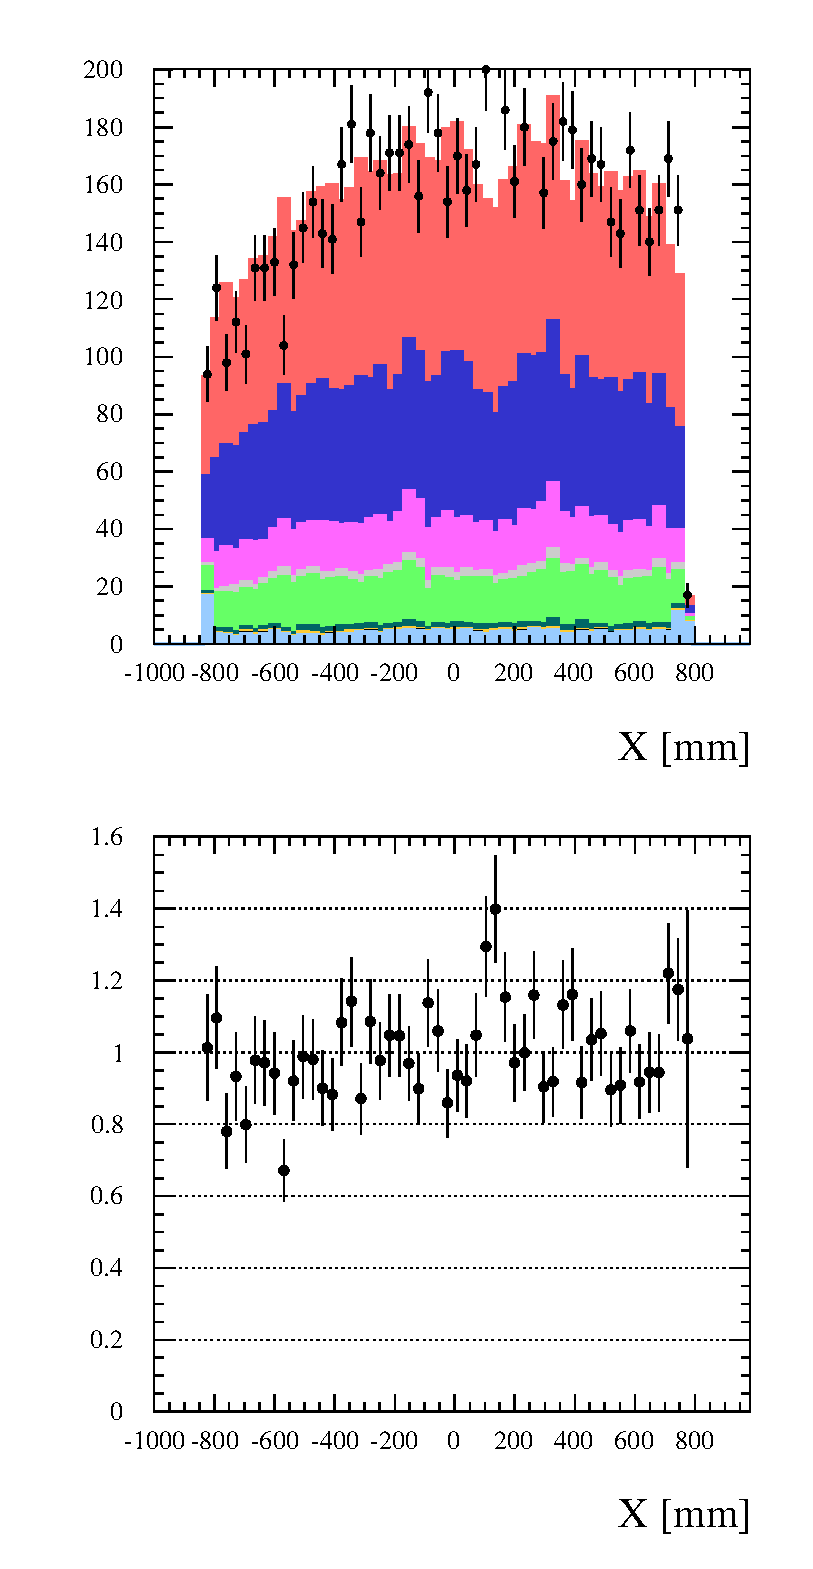
\includegraphics[width=3in]{Figures/P0DTrkXRun1Run2-normByRatio.eps}
  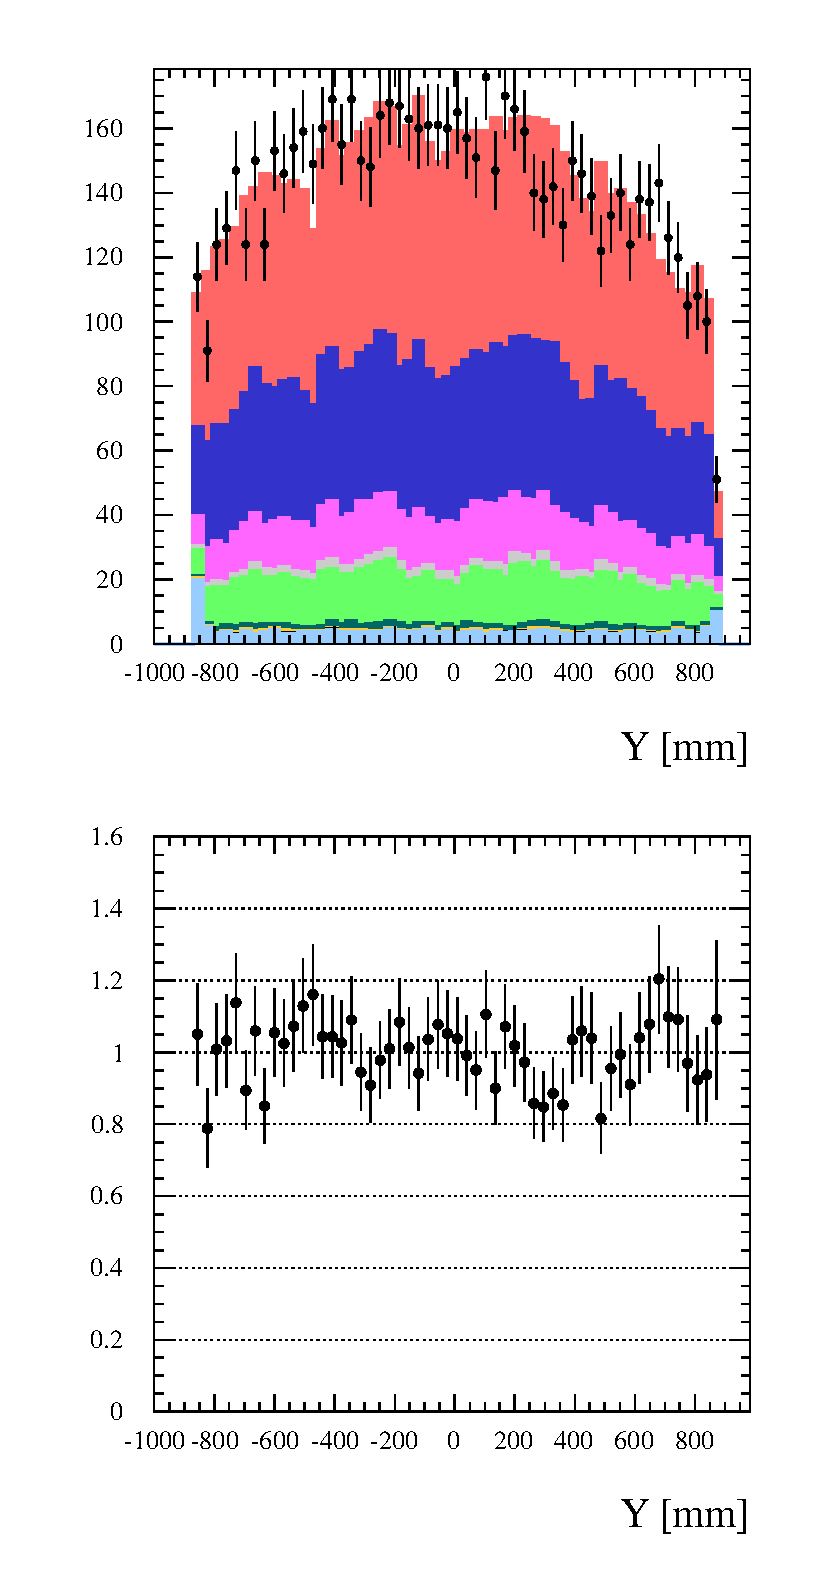
\includegraphics[width=3in]{Figures/P0DTrkYRun1Run2-normByRatio.eps}
  \caption{The candidate muon track start X and Y distributions 
Data to MC plots normalized by area.}
%Momentum (top left), (Cos Theta)THETA (top right), Phi (bottom left), and Z Vertex Position (bottom right) of the Muon candidate track for (Run 1)RUN1+RUN2. All corrections and reweighting have been applied.} 
  \label{fig:ResultsNorm}%FIXME
\end{figure}

\begin{figure}[h]
  \centering
  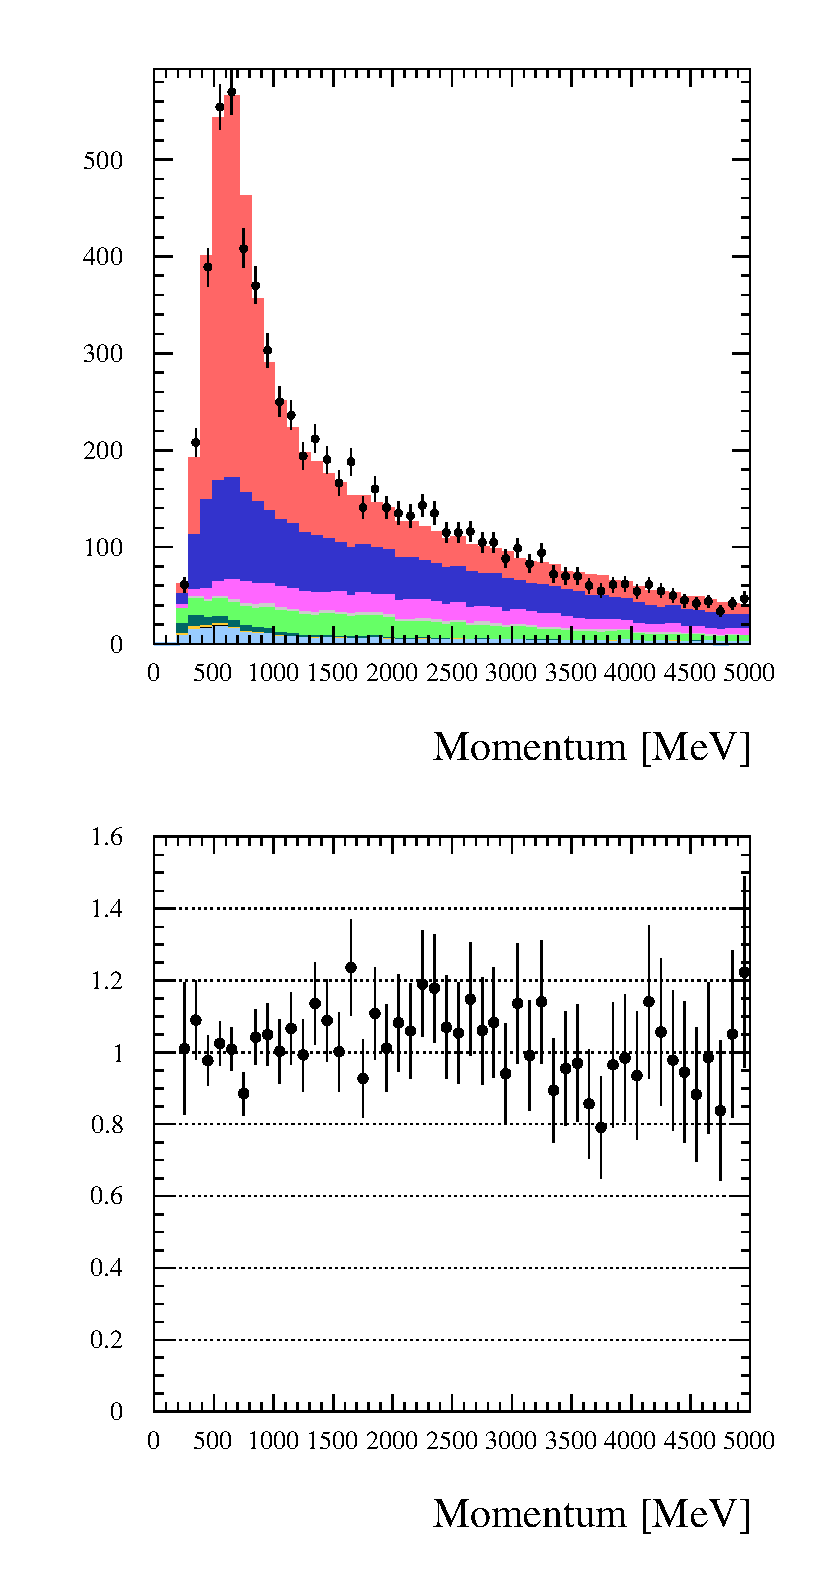
\includegraphics[width=3in]{Figures/P0DTrackerMomRun1Run2-normByRatio.eps}
  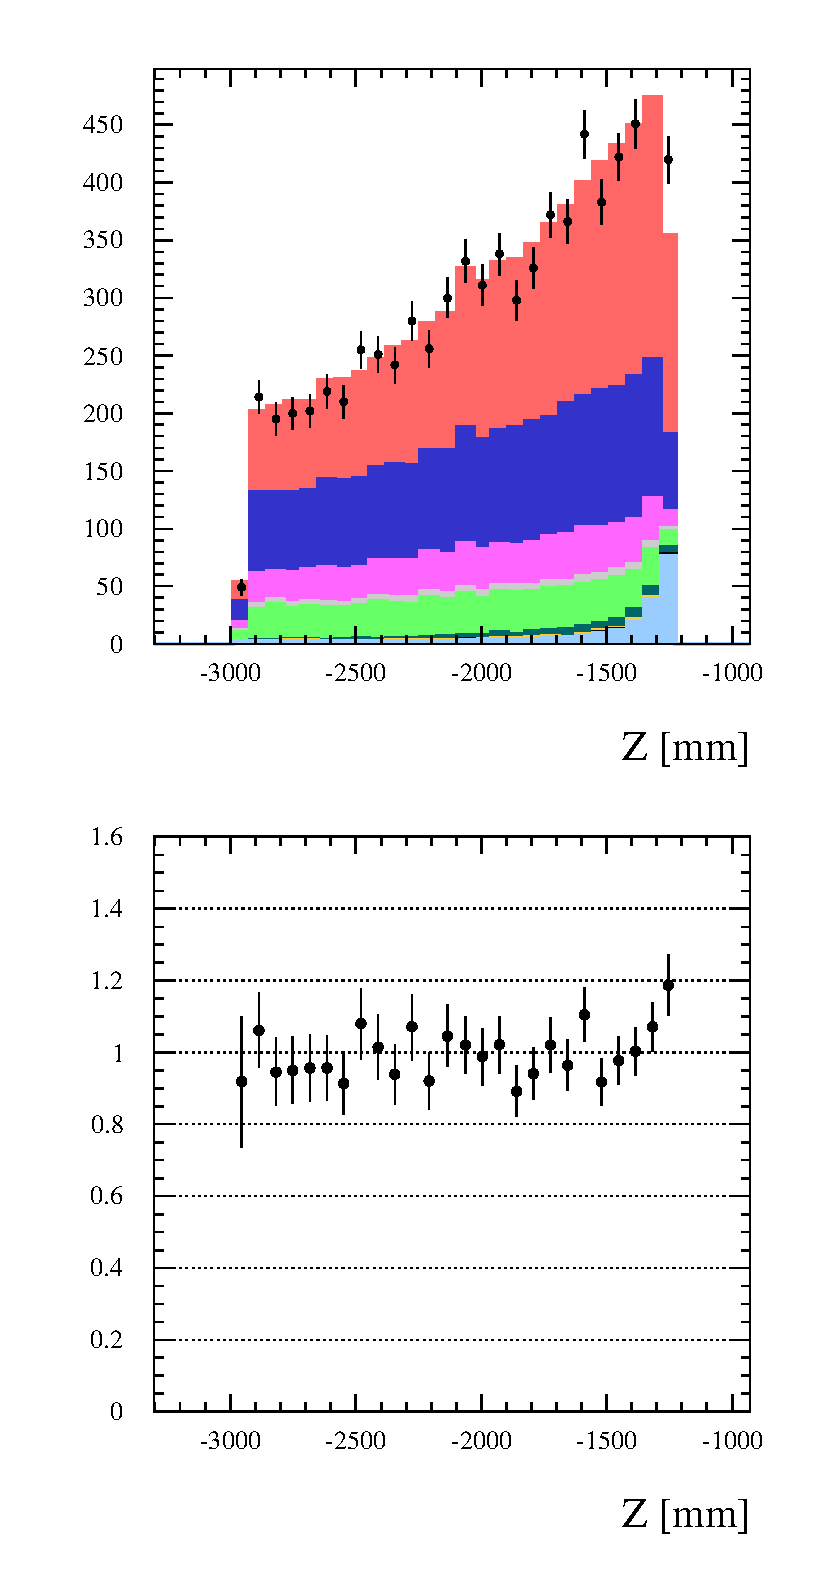
\includegraphics[width=3in]{Figures/P0DTrkZRun1Run2-normByRatio.eps}
  \caption{The candidate muon track Momentum and start Z distributions 
Data to MC plots normalized by area.}
%Momentum (top left), (Cos Theta)THETA (top right), Phi (bottom left), and Z Vertex Position (bottom right) of the Muon candidate track for (Run 1)RUN1+RUN2. All corrections and reweighting have been applied.} 
  \label{fig:ResultsNorm}%FIXME
\end{figure}

\begin{figure}[h]
  \centering
  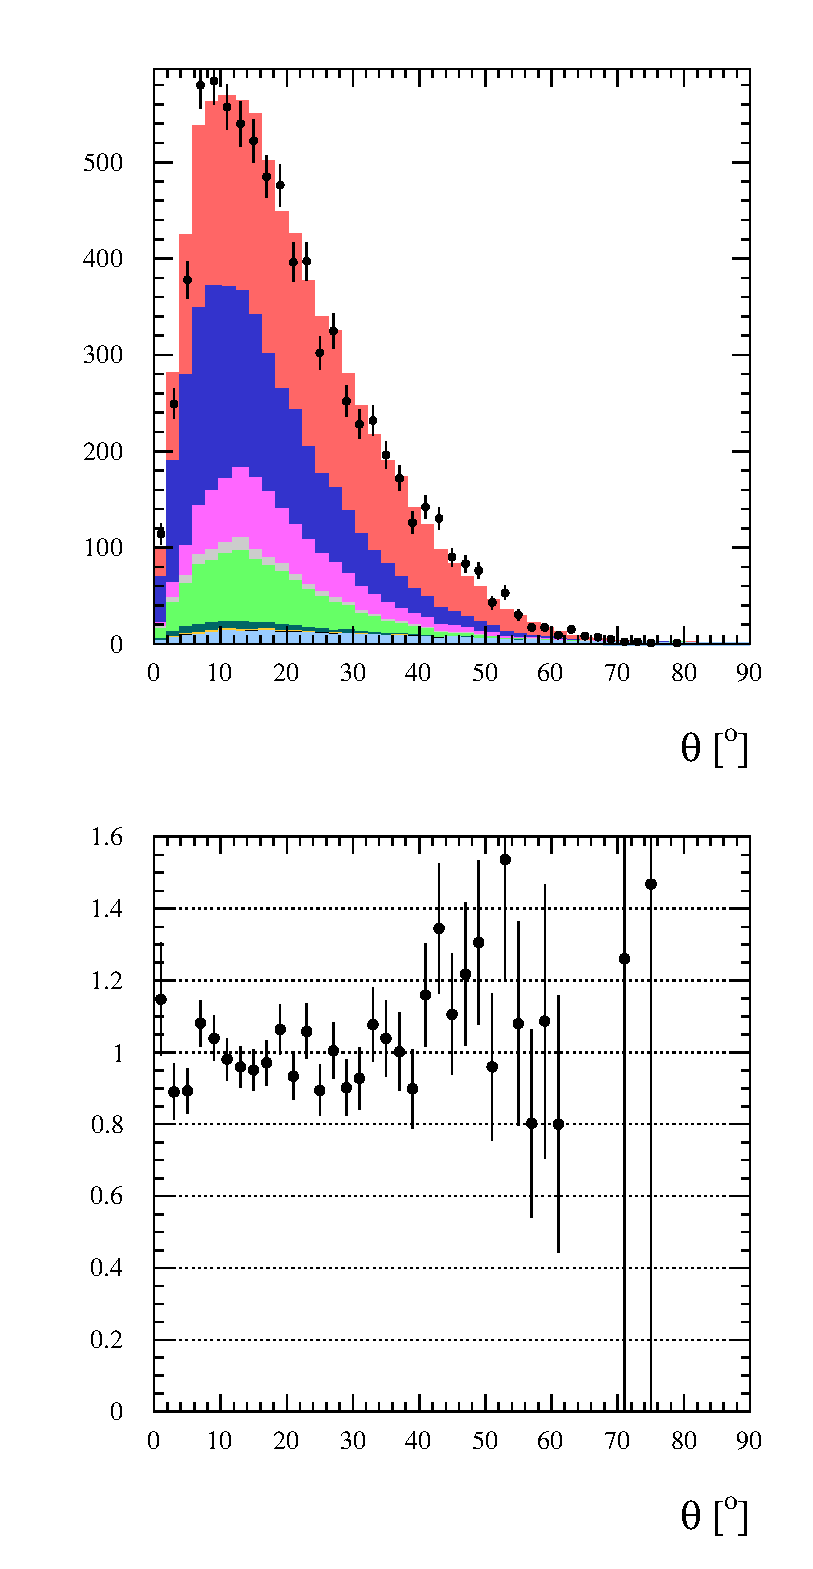
\includegraphics[width=3in]{Figures/P0DTrkThetaRun1Run2-normByRatio.eps}
  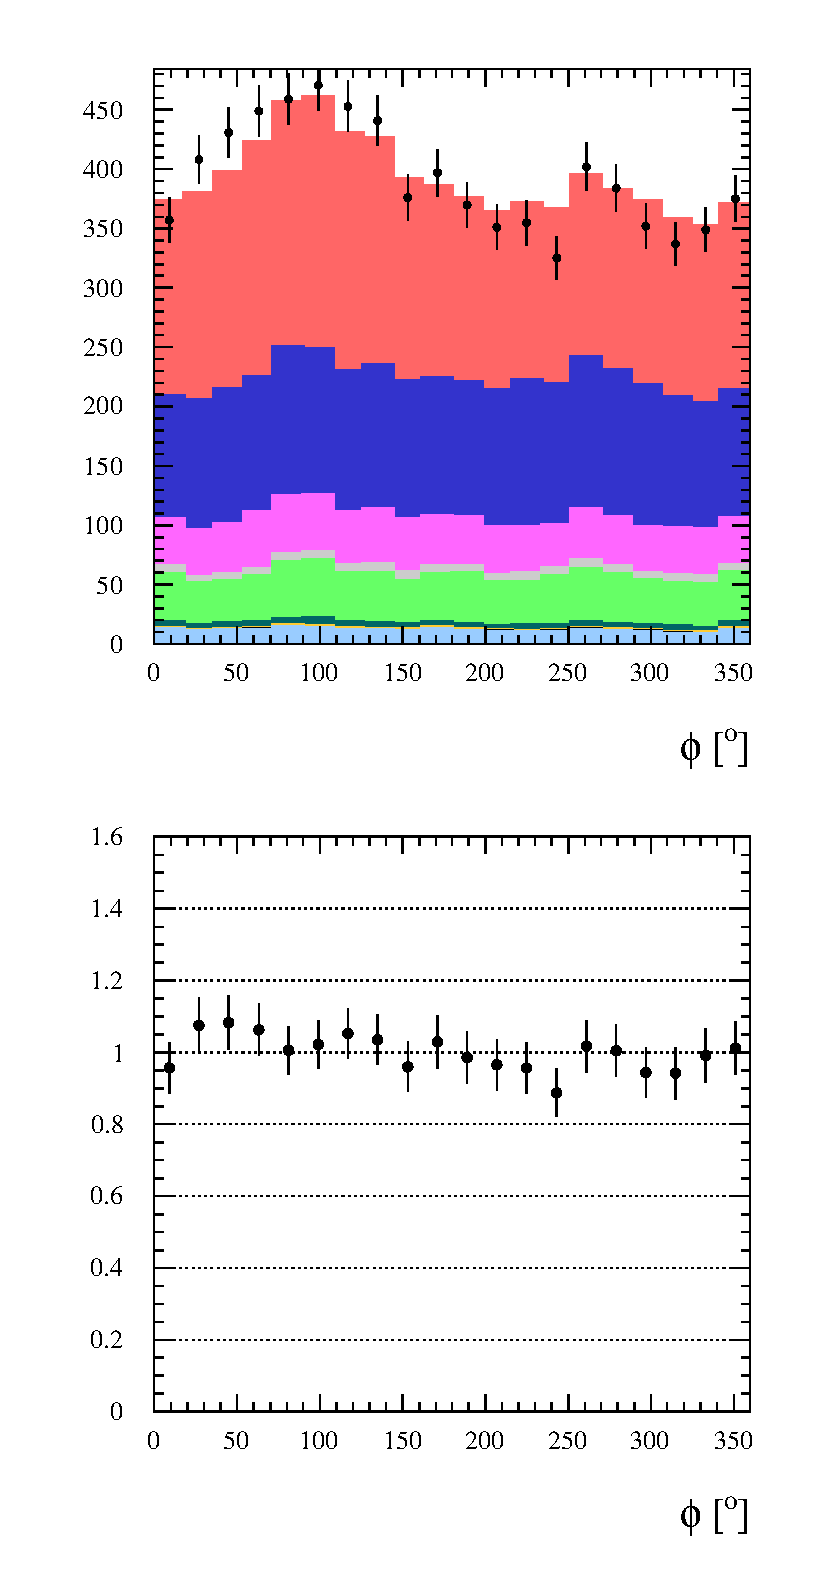
\includegraphics[width=3in]{Figures/P0DTrkPhiRun1Run2-normByRatio.eps}
  \caption{The candidate muon track start $\theta$ and $\phi$ distributions 
Data to MC plots normalized by area.}
%Momentum (top left), (Cos Theta)THETA (top right), Phi (bottom left), and Z Vertex Position (bottom right) of the Muon candidate track for (Run 1)RUN1+RUN2. All corrections and reweighting have been applied.} 
  \label{fig:ResultsNorm}%FIXME
\end{figure}
